\specialchapter{\texorpdfstring{PLATE I. SYSTEMS OF TYPE \(\mathbf{A}_l\) (\(l \geqslant 1\))}{PLATE I. SYSTEMS OF TYPE A\_l (l >= 1)}}

\begin{enumerate}
\def\labelenumi{(\Roman{enumi})}
\tightlist
\item
  V is the hyperplane of \(\mathbf{E} = \mathbf{R}^{l + 1}\) consisting of the points the sum of whose coordinates is zero.
\end{enumerate}

Roots: \(\varepsilon_{i} - \varepsilon_{j}\) ( \(i \neq j, 1 \leqslant i \leqslant l + 1, 1 \leqslant j \leqslant l + 1\) ).

Number of roots: \(n = l(l + 1)\) .

\begin{enumerate}
\def\labelenumi{(\Roman{enumi})}
\setcounter{enumi}{1}
\item
  Basis: \(\alpha_{1} = \varepsilon_{1} - \varepsilon_{2},\alpha_{2} = \varepsilon_{2} - \varepsilon_{3},\ldots ,\alpha_{l} = \varepsilon_{l} - \varepsilon_{l + 1}\) . Positive roots: \(\varepsilon_{i} - \varepsilon_{j} = \sum_{i\leqslant k <   j}\alpha_{k}\) ( \(1\leqslant i <   j\leqslant l + 1\) ).
\item
  Coxeter number: \(h = l + 1\) .
\item
  Highest root: \(\tilde{\alpha} = \varepsilon_{1} - \varepsilon_{l+1} = \alpha_{1} + \alpha_{2} + \cdots + \alpha_{l} = \omega_{1} + \omega_{l}\) . Completed Dynkin graph ( \(l \geqslant 2\) ):
\end{enumerate}

\pandocbounded{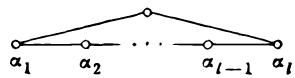
\includegraphics[keepaspectratio]{images/part002_112fabda.jpg}}

For \(l = 1\) , the Coxeter graph of the affine Weyl group is

\pandocbounded{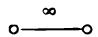
\includegraphics[keepaspectratio]{images/part002_c1e413d9.jpg}}

\begin{enumerate}
\def\labelenumi{(\Alph{enumi})}
\setcounter{enumi}{21}
\tightlist
\item
  \(R^{\prime} = R,\)
\end{enumerate}

\[
\Phi_ {\mathrm{R}} (x, y) = \frac {(x | y)}{2 (l + 1)}, \quad \gamma (\mathrm{R}) = (l + 1) ^ {2}.
\]

\begin{enumerate}
\def\labelenumi{(\Roman{enumi})}
\setcounter{enumi}{5}
\tightlist
\item
  Fundamental weights:
\end{enumerate}

\[
\begin{array}{l} \omega_ {i} = \varepsilon_ {1} + \dots + \varepsilon_ {i} - \frac {i}{l + 1} \sum_ {j = 1} ^ {l + 1} \varepsilon_ {j} \\ = \frac {1}{l + 1} [ (l - i + 1) (\alpha_ {1} + 2 \alpha_ {2} + \dots + (i - 1) \alpha_ {i - 1}) \\ \qquad + i ((l - i + 1) \alpha_ {i} + (l - i) \alpha_ {i + 1} + \dots + \alpha_ {l}) ]. \end{array}
\]

\begin{enumerate}
\def\labelenumi{(\Roman{enumi})}
\setcounter{enumi}{6}
\tightlist
\item
  Sum of the positive roots:
\end{enumerate}

\[
\begin{array}{c} 2 \rho = l \varepsilon_ {1} + (l - 2) \varepsilon_ {2} + (l - 4) \varepsilon_ {3} + \dots - (l - 2) \varepsilon_ {l} - l \varepsilon_ {l + 1} \\ = l \alpha_ {1} + 2 (l - 1) \alpha_ {2} + \dots + i (l - i + 1) \alpha_ {i} + \dots + l \alpha_ {l}. \end{array}
\]

\begin{enumerate}
\def\labelenumi{(\Roman{enumi})}
\setcounter{enumi}{7}
\item
  Q(R): the set of vectors whose coordinates are integers with sum zero. P(R): generated by Q(R) and \(\varepsilon_{1} - (l + 1)^{-1}(\varepsilon_{1} + \varepsilon_{2} + \cdots + \varepsilon_{l+1})\) . P(R)/Q(R) is isomorphic to Z/(l+1)Z. Connection index: l + 1.
\item
  Exponents: 1, 2, \ldots, l.
\item
  \(\mathrm{W}(\mathrm{R}) = \mathfrak{S}_{l + 1}\) , identified with the group of permutations of the \(\varepsilon_{i}\) . Order of \(\mathrm{W}(\mathrm{R})\colon (l + 1)!\)
\item
  \(l = 1\) : A(R) = W(R); \(w_0 = -1\) .
\end{enumerate}

\(l \geqslant 2: A(R) = W(R) \times \{1, -1\} \text{ and } w_{0} \text{ transforms } \alpha_{i} \text{ to } -\alpha_{l+1-i}.\)

\begin{enumerate}
\def\labelenumi{(\Roman{enumi})}
\setcounter{enumi}{11}
\item
  The group \(\mathrm{P}(\mathrm{R}^{-})/\mathrm{Q}(\mathrm{R}^{-})\) is cyclic of order \((l+1)\) ; it acts on the completed Dynkin graph by circular permutations. If \(l \geqslant 2\) , the unique non-identity element of \(\mathrm{A}(\mathrm{R})/\mathrm{W}(\mathrm{R})\) acts on \(\mathrm{P}(\mathrm{R})/\mathrm{Q}(\mathrm{R})\) by the automorphism \(x \mapsto -x\) .
\item
  Cartan matrix \((l \times l)\) :
\end{enumerate}

\[
\left( \begin{array}{c c c c c c c} 2 & - 1 & 0 & 0 & \dots & 0 & 0 \\ - 1 & 2 & - 1 & 0 & \dots & 0 & 0 \\ 0 & - 1 & 2 & - 1 & \dots & 0 & 0 \\ 0 & 0 & - 1 & 2 & \dots & 0 & 0 \\ \vdots & \vdots & \vdots & \vdots & \ddots & \vdots & \vdots \\ 0 & 0 & 0 & 0 & \dots & - 1 & 2 \end{array} \right)
\]

